% Options for packages loaded elsewhere
\PassOptionsToPackage{unicode}{hyperref}
\PassOptionsToPackage{hyphens}{url}
%
\documentclass[
]{article}
\usepackage{amsmath,amssymb}
\usepackage{lmodern}
\usepackage{ifxetex,ifluatex}
\ifnum 0\ifxetex 1\fi\ifluatex 1\fi=0 % if pdftex
  \usepackage[T1]{fontenc}
  \usepackage[utf8]{inputenc}
  \usepackage{textcomp} % provide euro and other symbols
\else % if luatex or xetex
  \usepackage{unicode-math}
  \defaultfontfeatures{Scale=MatchLowercase}
  \defaultfontfeatures[\rmfamily]{Ligatures=TeX,Scale=1}
\fi
% Use upquote if available, for straight quotes in verbatim environments
\IfFileExists{upquote.sty}{\usepackage{upquote}}{}
\IfFileExists{microtype.sty}{% use microtype if available
  \usepackage[]{microtype}
  \UseMicrotypeSet[protrusion]{basicmath} % disable protrusion for tt fonts
}{}
\makeatletter
\@ifundefined{KOMAClassName}{% if non-KOMA class
  \IfFileExists{parskip.sty}{%
    \usepackage{parskip}
  }{% else
    \setlength{\parindent}{0pt}
    \setlength{\parskip}{6pt plus 2pt minus 1pt}}
}{% if KOMA class
  \KOMAoptions{parskip=half}}
\makeatother
\usepackage{xcolor}
\IfFileExists{xurl.sty}{\usepackage{xurl}}{} % add URL line breaks if available
\IfFileExists{bookmark.sty}{\usepackage{bookmark}}{\usepackage{hyperref}}
\hypersetup{
  pdftitle={Analysis for CCFP paper},
  pdfauthor={Peter S. Hovmand},
  hidelinks,
  pdfcreator={LaTeX via pandoc}}
\urlstyle{same} % disable monospaced font for URLs
\usepackage[margin=1in]{geometry}
\usepackage{color}
\usepackage{fancyvrb}
\newcommand{\VerbBar}{|}
\newcommand{\VERB}{\Verb[commandchars=\\\{\}]}
\DefineVerbatimEnvironment{Highlighting}{Verbatim}{commandchars=\\\{\}}
% Add ',fontsize=\small' for more characters per line
\usepackage{framed}
\definecolor{shadecolor}{RGB}{248,248,248}
\newenvironment{Shaded}{\begin{snugshade}}{\end{snugshade}}
\newcommand{\AlertTok}[1]{\textcolor[rgb]{0.94,0.16,0.16}{#1}}
\newcommand{\AnnotationTok}[1]{\textcolor[rgb]{0.56,0.35,0.01}{\textbf{\textit{#1}}}}
\newcommand{\AttributeTok}[1]{\textcolor[rgb]{0.77,0.63,0.00}{#1}}
\newcommand{\BaseNTok}[1]{\textcolor[rgb]{0.00,0.00,0.81}{#1}}
\newcommand{\BuiltInTok}[1]{#1}
\newcommand{\CharTok}[1]{\textcolor[rgb]{0.31,0.60,0.02}{#1}}
\newcommand{\CommentTok}[1]{\textcolor[rgb]{0.56,0.35,0.01}{\textit{#1}}}
\newcommand{\CommentVarTok}[1]{\textcolor[rgb]{0.56,0.35,0.01}{\textbf{\textit{#1}}}}
\newcommand{\ConstantTok}[1]{\textcolor[rgb]{0.00,0.00,0.00}{#1}}
\newcommand{\ControlFlowTok}[1]{\textcolor[rgb]{0.13,0.29,0.53}{\textbf{#1}}}
\newcommand{\DataTypeTok}[1]{\textcolor[rgb]{0.13,0.29,0.53}{#1}}
\newcommand{\DecValTok}[1]{\textcolor[rgb]{0.00,0.00,0.81}{#1}}
\newcommand{\DocumentationTok}[1]{\textcolor[rgb]{0.56,0.35,0.01}{\textbf{\textit{#1}}}}
\newcommand{\ErrorTok}[1]{\textcolor[rgb]{0.64,0.00,0.00}{\textbf{#1}}}
\newcommand{\ExtensionTok}[1]{#1}
\newcommand{\FloatTok}[1]{\textcolor[rgb]{0.00,0.00,0.81}{#1}}
\newcommand{\FunctionTok}[1]{\textcolor[rgb]{0.00,0.00,0.00}{#1}}
\newcommand{\ImportTok}[1]{#1}
\newcommand{\InformationTok}[1]{\textcolor[rgb]{0.56,0.35,0.01}{\textbf{\textit{#1}}}}
\newcommand{\KeywordTok}[1]{\textcolor[rgb]{0.13,0.29,0.53}{\textbf{#1}}}
\newcommand{\NormalTok}[1]{#1}
\newcommand{\OperatorTok}[1]{\textcolor[rgb]{0.81,0.36,0.00}{\textbf{#1}}}
\newcommand{\OtherTok}[1]{\textcolor[rgb]{0.56,0.35,0.01}{#1}}
\newcommand{\PreprocessorTok}[1]{\textcolor[rgb]{0.56,0.35,0.01}{\textit{#1}}}
\newcommand{\RegionMarkerTok}[1]{#1}
\newcommand{\SpecialCharTok}[1]{\textcolor[rgb]{0.00,0.00,0.00}{#1}}
\newcommand{\SpecialStringTok}[1]{\textcolor[rgb]{0.31,0.60,0.02}{#1}}
\newcommand{\StringTok}[1]{\textcolor[rgb]{0.31,0.60,0.02}{#1}}
\newcommand{\VariableTok}[1]{\textcolor[rgb]{0.00,0.00,0.00}{#1}}
\newcommand{\VerbatimStringTok}[1]{\textcolor[rgb]{0.31,0.60,0.02}{#1}}
\newcommand{\WarningTok}[1]{\textcolor[rgb]{0.56,0.35,0.01}{\textbf{\textit{#1}}}}
\usepackage{graphicx}
\makeatletter
\def\maxwidth{\ifdim\Gin@nat@width>\linewidth\linewidth\else\Gin@nat@width\fi}
\def\maxheight{\ifdim\Gin@nat@height>\textheight\textheight\else\Gin@nat@height\fi}
\makeatother
% Scale images if necessary, so that they will not overflow the page
% margins by default, and it is still possible to overwrite the defaults
% using explicit options in \includegraphics[width, height, ...]{}
\setkeys{Gin}{width=\maxwidth,height=\maxheight,keepaspectratio}
% Set default figure placement to htbp
\makeatletter
\def\fps@figure{htbp}
\makeatother
\setlength{\emergencystretch}{3em} % prevent overfull lines
\providecommand{\tightlist}{%
  \setlength{\itemsep}{0pt}\setlength{\parskip}{0pt}}
\setcounter{secnumdepth}{-\maxdimen} % remove section numbering
\ifluatex
  \usepackage{selnolig}  % disable illegal ligatures
\fi

\title{Analysis for CCFP paper}
\author{Peter S. Hovmand}
\date{Feb 27, 2022}

\begin{document}
\maketitle

\hypertarget{overview}{%
\subsection{Overview}\label{overview}}

This document was written and generated as an R Markdown document and
exported to Word. The document includes all the code and results for
replicating the results in the paper.

\hypertarget{requirements}{%
\subsection{Requirements}\label{requirements}}

The following are required for replicating this simulation study:

\begin{enumerate}
\def\labelenumi{\arabic{enumi}.}
\tightlist
\item
  Stella Architect (2.1.1 or higher) or Stella Simulator (2.1.1 or
  higher)
\item
  R (available at \url{https://cran.r-project.org/})
\item
  RStudio (available at \url{https://www.rstudio.com/})
\item
  Developmental-Transitions-2-2-9.stmx model
\end{enumerate}

\begin{Shaded}
\begin{Highlighting}[]
\FunctionTok{require}\NormalTok{(readr)    }\CommentTok{\# package for reading in csv files as tibble data frame}
\end{Highlighting}
\end{Shaded}

\begin{verbatim}
## Loading required package: readr
\end{verbatim}

\begin{Shaded}
\begin{Highlighting}[]
\FunctionTok{require}\NormalTok{(readxl)   }\CommentTok{\# reads Excel worksheets}
\end{Highlighting}
\end{Shaded}

\begin{verbatim}
## Loading required package: readxl
\end{verbatim}

\begin{Shaded}
\begin{Highlighting}[]
\FunctionTok{require}\NormalTok{(dplyr)    }\CommentTok{\# for manipulating data frames, etc. }
\end{Highlighting}
\end{Shaded}

\begin{verbatim}
## Loading required package: dplyr
\end{verbatim}

\begin{verbatim}
## 
## Attaching package: 'dplyr'
\end{verbatim}

\begin{verbatim}
## The following objects are masked from 'package:stats':
## 
##     filter, lag
\end{verbatim}

\begin{verbatim}
## The following objects are masked from 'package:base':
## 
##     intersect, setdiff, setequal, union
\end{verbatim}

\begin{Shaded}
\begin{Highlighting}[]
\FunctionTok{require}\NormalTok{(ggplot2)  }\CommentTok{\# for creating interactive plots }
\end{Highlighting}
\end{Shaded}

\begin{verbatim}
## Loading required package: ggplot2
\end{verbatim}

\begin{Shaded}
\begin{Highlighting}[]
\FunctionTok{require}\NormalTok{(reshape2) }\CommentTok{\# needed to reshape data for plotting with ggplot2}
\end{Highlighting}
\end{Shaded}

\begin{verbatim}
## Loading required package: reshape2
\end{verbatim}

\hypertarget{setting-up-individual-cases}{%
\subsection{Setting up individual
cases}\label{setting-up-individual-cases}}

The individual cases were generated by interactively varying the
parameters and initial conditions to generate a representative set of
developmental trajectories for cognitive vulnerabilities and family
support. The values for initial conditions and parameters for each case
were then exported from Stella Architect into an Excel worksheet that
can be read by R. Having the values in an external file provides a
flexible approach to add/modify cases as the model develops and
replicate the analyses.

\begin{Shaded}
\begin{Highlighting}[]
\CommentTok{\# read in the Excel file}
\NormalTok{cases.df }\OtherTok{\textless{}{-}} \FunctionTok{read\_excel}\NormalTok{(}\StringTok{"Cases.xlsx"}\NormalTok{)}

\CommentTok{\# print values of parameters and initial conditions used for each case}
\NormalTok{cases.df}
\end{Highlighting}
\end{Shaded}

\begin{verbatim}
## # A tibble: 6 x 7
##    Case Cognitive_Vulnera~ Family_Response_~ Family_Support_~ Initial_Cognitive~
##   <dbl>              <dbl>             <dbl>            <dbl>              <dbl>
## 1     1              0.125             0.125            0.125                 25
## 2     2              0.5              25               25                     25
## 3     3              1.25              0.1             12                     25
## 4     4              2                25               25                     25
## 5     5              2                25               25                     25
## 6     6              2                25               25                     25
## # ... with 2 more variables: Initial_Family_Support <dbl>,
## #   Onset_of_Maladaptive_Behaviors_Delay <dbl>
\end{verbatim}

\begin{Shaded}
\begin{Highlighting}[]
\CommentTok{\# create a vector that can be used later to iterate through the cases for }
\CommentTok{\# simulation, plotting, etc}
\NormalTok{cases.vec}\OtherTok{\textless{}{-}}\DecValTok{1}\SpecialCharTok{:}\FunctionTok{nrow}\NormalTok{(cases.df) }
\end{Highlighting}
\end{Shaded}

\hypertarget{simulate-a-baserun-for-each-case}{%
\subsection{Simulate a baserun for each
case}\label{simulate-a-baserun-for-each-case}}

The baserun for each case is simulated with the results imported via a
.csv file and saved in the dataframe results.baserun.

\begin{Shaded}
\begin{Highlighting}[]
\NormalTok{results.baseruns }\OtherTok{\textless{}{-}} \ConstantTok{NULL} \CommentTok{\# create an empty objects to store results}

\CommentTok{\# iterate over the list of cases }
\ControlFlowTok{for}\NormalTok{ (i }\ControlFlowTok{in}\NormalTok{ cases.vec) \{}
  \CommentTok{\# print progress}
  \FunctionTok{cat}\NormalTok{(}\StringTok{"Case ="}\NormalTok{,i,}\StringTok{"}\SpecialCharTok{\textbackslash{}n}\StringTok{"}\NormalTok{)}
  
  \CommentTok{\# pull the parameters from the row in the case data frame}
\NormalTok{  parms }\OtherTok{\textless{}{-}}\NormalTok{ cases.df }\SpecialCharTok{\%\textgreater{}\%}            \CommentTok{\# start wtih the data frame}
            \FunctionTok{filter}\NormalTok{(Case}\SpecialCharTok{==}\NormalTok{i) }\SpecialCharTok{\%\textgreater{}\%}    \CommentTok{\# select row for case = i }
            \FunctionTok{select}\NormalTok{(}\SpecialCharTok{!}\NormalTok{Case)          }\CommentTok{\# drop the Case column}
  
  \CommentTok{\# write the parameters to the Stella import file}
  \FunctionTok{write\_csv}\NormalTok{(parms, }\AttributeTok{file=}\StringTok{"Parms.csv"}\NormalTok{)}
  
  \CommentTok{\# run the simulation }
  \FunctionTok{system2}\NormalTok{(}\StringTok{"stella\_simulator"}\NormalTok{,}
        \AttributeTok{args =} \StringTok{"{-}r Developmental{-}Transitions{-}2{-}2{-}10.stmx"}\NormalTok{,}
        \AttributeTok{env =} \StringTok{"PATH=$PATH:/Applications/Stella\_Simulator"}\NormalTok{, }
        \AttributeTok{wait=}\ConstantTok{TRUE}\NormalTok{)}
  
  \CommentTok{\# read the results and add them to the data frame}
  
\NormalTok{  results.baseruns}\OtherTok{\textless{}{-}}\FunctionTok{rbind}\NormalTok{(results.baseruns, }
                          \FunctionTok{tibble}\NormalTok{(}\AttributeTok{Case=}\NormalTok{i,}\FunctionTok{read\_csv}\NormalTok{(}\StringTok{"Results.csv"}\NormalTok{)))}
  
\NormalTok{\}}
\end{Highlighting}
\end{Shaded}

\begin{verbatim}
## Case = 1 
## Case = 2 
## Case = 3 
## Case = 4 
## Case = 5 
## Case = 6
\end{verbatim}

\hypertarget{plot-results}{%
\subsection{Plot results}\label{plot-results}}

Results are plotted using \texttt{ggplot2} package showing the dynamics
of cognitive vulnerabilities and family support for each hypothetical
case.

\begin{Shaded}
\begin{Highlighting}[]
\CommentTok{\# Select a vector of time points to plot}
\NormalTok{t.plot }\OtherTok{\textless{}{-}} \FunctionTok{unique}\NormalTok{(results.baseruns}\SpecialCharTok{$}\NormalTok{Years)}
\NormalTok{t.plot }\OtherTok{\textless{}{-}}\NormalTok{ t.plot[}\FunctionTok{seq}\NormalTok{(}\DecValTok{1}\NormalTok{,}\FunctionTok{length}\NormalTok{(t.plot),}\DecValTok{100}\NormalTok{)]}

\CommentTok{\# Plot the results}
\NormalTok{results.baseruns }\SpecialCharTok{\%\textgreater{}\%} 
  \FunctionTok{select}\NormalTok{(Case, Years, }\StringTok{\textasciigrave{}}\AttributeTok{Cognitive Vulnerabilities}\StringTok{\textasciigrave{}}\NormalTok{, }\StringTok{\textasciigrave{}}\AttributeTok{Family Support}\StringTok{\textasciigrave{}}\NormalTok{) }\SpecialCharTok{\%\textgreater{}\%}
  \FunctionTok{filter}\NormalTok{(Years }\SpecialCharTok{\%in\%}\NormalTok{ t.plot) }\SpecialCharTok{\%\textgreater{}\%}
  \FunctionTok{melt}\NormalTok{(}\AttributeTok{id=}\FunctionTok{c}\NormalTok{(}\StringTok{"Case"}\NormalTok{,}\StringTok{"Years"}\NormalTok{)) }\SpecialCharTok{\%\textgreater{}\%} 
    \FunctionTok{ggplot}\NormalTok{(}\FunctionTok{aes}\NormalTok{(}\AttributeTok{x=}\NormalTok{Years, }\AttributeTok{y=}\NormalTok{value)) }\SpecialCharTok{+}
    \FunctionTok{geom\_line}\NormalTok{(}\FunctionTok{aes}\NormalTok{(}\AttributeTok{linetype =}\NormalTok{ variable)) }\SpecialCharTok{+}
    \FunctionTok{ylab}\NormalTok{(}\StringTok{""}\NormalTok{) }\SpecialCharTok{+} 
    \FunctionTok{xlab}\NormalTok{(}\StringTok{"Age"}\NormalTok{) }\SpecialCharTok{+}
    \FunctionTok{facet\_wrap}\NormalTok{(}\SpecialCharTok{\textasciitilde{}}\NormalTok{Case) }\SpecialCharTok{+}
    \FunctionTok{theme\_bw}\NormalTok{() }\SpecialCharTok{+}
    \FunctionTok{theme}\NormalTok{(}\AttributeTok{legend.position =} \StringTok{"bottom"}\NormalTok{, }
          \AttributeTok{legend.title =} \FunctionTok{element\_blank}\NormalTok{())}
\end{Highlighting}
\end{Shaded}

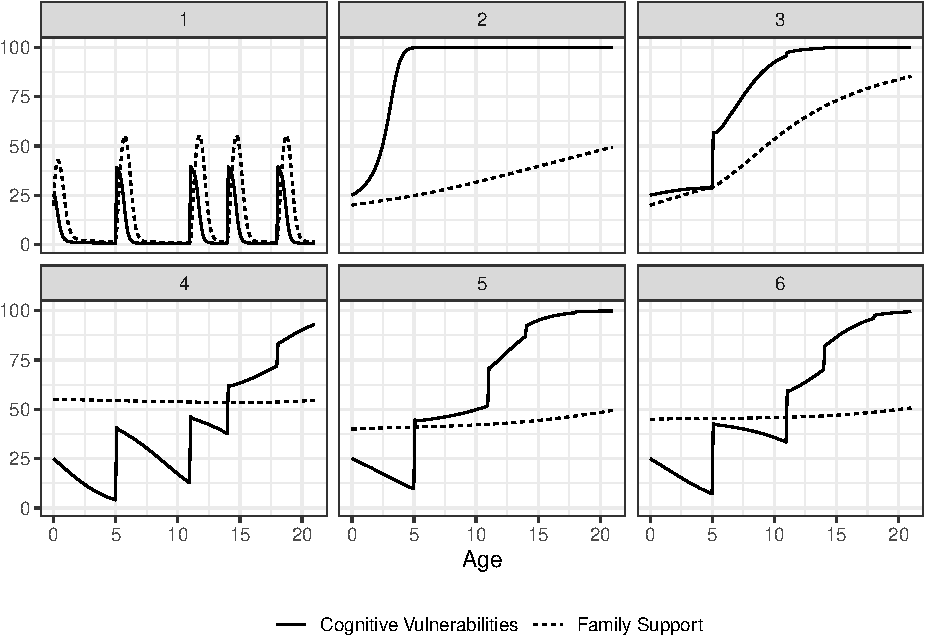
\includegraphics{Study-1_files/figure-latex/plot each case using ggplot2-1.pdf}

Loop scores for each of the three major loops are then plotted for each
case.

\begin{Shaded}
\begin{Highlighting}[]
\NormalTok{results.baseruns }\SpecialCharTok{\%\textgreater{}\%} 
  \FunctionTok{select}\NormalTok{(Case, Years, }\StringTok{\textasciigrave{}}\AttributeTok{R1 Loop Score}\StringTok{\textasciigrave{}}\NormalTok{, }\StringTok{\textasciigrave{}}\AttributeTok{B1 Loop Score}\StringTok{\textasciigrave{}}\NormalTok{, }\StringTok{\textasciigrave{}}\AttributeTok{B2 Loop Score}\StringTok{\textasciigrave{}}\NormalTok{) }\SpecialCharTok{\%\textgreater{}\%}
  \FunctionTok{filter}\NormalTok{(Years }\SpecialCharTok{\%in\%}\NormalTok{ t.plot) }\SpecialCharTok{\%\textgreater{}\%}
  \FunctionTok{melt}\NormalTok{(}\AttributeTok{id=}\FunctionTok{c}\NormalTok{(}\StringTok{"Case"}\NormalTok{,}\StringTok{"Years"}\NormalTok{)) }\SpecialCharTok{\%\textgreater{}\%} 
    \FunctionTok{ggplot}\NormalTok{(}\FunctionTok{aes}\NormalTok{(}\AttributeTok{x=}\NormalTok{Years, }\AttributeTok{y=}\NormalTok{value)) }\SpecialCharTok{+}
    \FunctionTok{geom\_line}\NormalTok{(}\FunctionTok{aes}\NormalTok{(}\AttributeTok{linetype =}\NormalTok{ variable)) }\SpecialCharTok{+}
    \FunctionTok{ylab}\NormalTok{(}\StringTok{"Normalized Loop Score"}\NormalTok{) }\SpecialCharTok{+} 
    \FunctionTok{xlab}\NormalTok{(}\StringTok{"Age"}\NormalTok{) }\SpecialCharTok{+} 
    \FunctionTok{facet\_wrap}\NormalTok{(}\SpecialCharTok{\textasciitilde{}}\NormalTok{Case) }\SpecialCharTok{+}
    \FunctionTok{theme\_bw}\NormalTok{() }\SpecialCharTok{+} 
    \FunctionTok{theme}\NormalTok{(}\AttributeTok{legend.position =} \StringTok{"bottom"}\NormalTok{, }
          \AttributeTok{legend.title =} \FunctionTok{element\_blank}\NormalTok{())}
\end{Highlighting}
\end{Shaded}

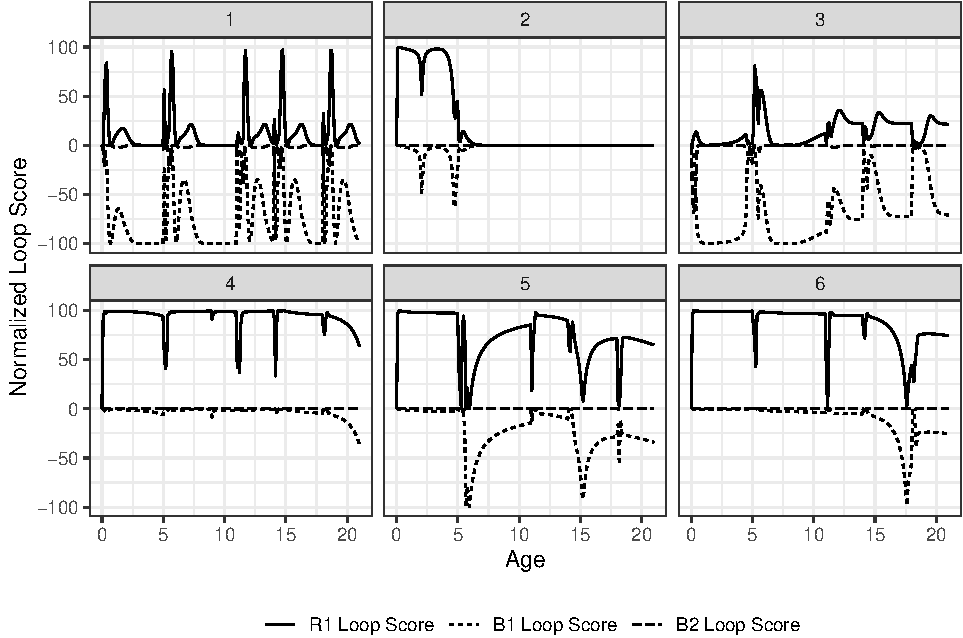
\includegraphics{Study-1_files/figure-latex/plot loop scores-1.pdf}

\end{document}
